%350

第2回で出てきた条件判断について思い出してみましょう。

プログラムは最初の行から、下に向かって\ruby{順番}{じゅん|ばん}に実行されます。\ruby{実際}{じっ|さい}には、\ruby{一瞬}{いっ|しゅん}ですぎてしまうのでわかりにくいですが、どのような順番でコンピューターが動くのか、想像しながら見てみることが大切です。わからない命令は以前の教科書を復習してみましょう。
\clearpage

「*hata」から「goto *hata」までの\ruby{間}{あいだ}が「スイッチ押して」という文字を\ruby{表示}{ひょう|じ}する部分です。




\begin{description}
    \item \textgt{\bf *hata}
    \item \textgt{\bf \ \ \ \ redraw 0}
    \item \textgt{\bf \ \ \ \ font {\textquotedbl}{\textquotedbl},60}
    \item \textgt{\bf \ \ \ \ pos 60,180}
    \item \textgt{\bf \ \ \ \ color 0,0,255}
    \item \textgt{\bf \ \ \ \ mes {\textquotedbl}スイッチ押して{\textquotedbl}}
    \item \textgt{\bf \ \ \ \ redraw 1}
    \item \textgt{\bf \ \ \ \ await 16}
    \item \textgt{\bf \ \ \ \ if gpioin(5)=0 : goto *hata2}
    \item \textgt{\bf \ \ \ \ goto *hata}
\end{description}

ここでセンサーボードのスイッチを押すと流れが変わります。

\begin{description}
    \item \textgt{\bf *hata2}
    \item \textgt{\bf \ \ \ \ redraw 0}
    \item \textgt{\bf \ \ \ \ font {\textquotedbl}{\textquotedbl},60}
    \item \textgt{\bf \ \ \ \ pos 60,180}
    \item \textgt{\bf \ \ \ \ color 255,0,0}
    \item \textgt{\bf \ \ \ \ mes {\textquotedbl}押しましたね!{\textquotedbl}}
    \item \textgt{\bf \ \ \ \ redraw 1}
    \item \textgt{\bf \ \ \ \ await 16}
    \item \textgt{\bf \ \ \ \ if gpioin(6)=0 : goto *hata}
    \item \textgt{\bf \ \ \ \ goto *hata2}
\end{description}


「*hata2」から「goto *hata2」までの間で「押しましたね」という文字を表示しています。

それぞれの\ruby{切}{き}り\ruby{替}{か}えにスイッチを使っていますが、そのために条件判断を使っています。

スイッチの\ruby{状態}{じょう|たい}などを知る\ruby{場合}{ば|あい}は、gpioinという\ruby{関数}{かん|すう}を使います。



\begin{description}
    \item \textgt{\bf \ \ 変数 = gpioin(GPIO番号)}
\end{description}

と書くことで、指定されたGPIO番号のスイッチがONかOFFかを調べることができます。

%444


\begin{figure}[H]
    \begin{center}
      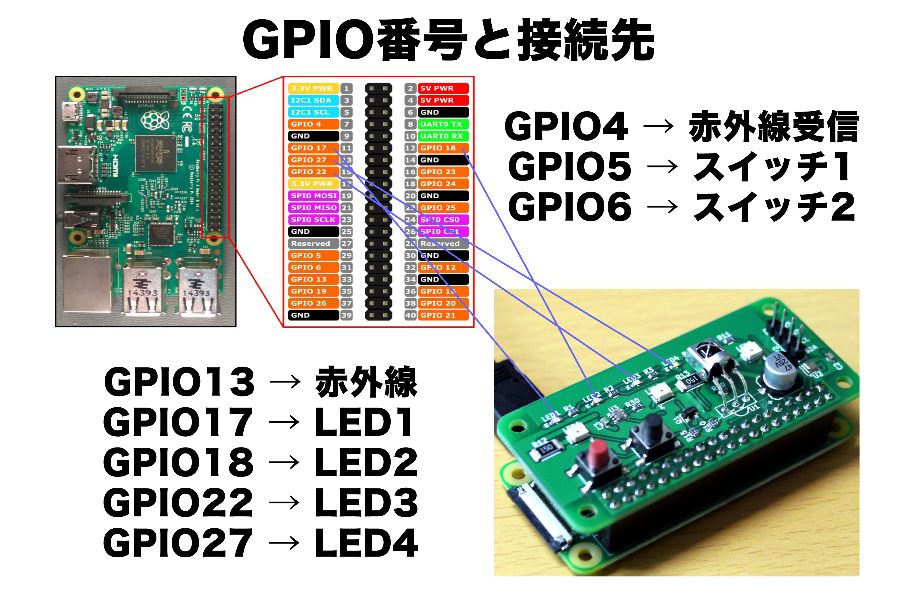
\includegraphics[keepaspectratio,width=12.409cm,height=7.62cm]{text04-img/text04-img004.png}
    \end{center}
    \label{fig:prog_menu}
\end{figure}



スイッチが接続されているGPIOの番号を指定することで\ruby{変数}{へん|すう}に値を入れることができます。

\begin{description}
    \item \textgt{\bf \ \ a = gpioin(5)}
\end{description}



と書くことで、スイッチ1がONならば0、OFFならば1が変数に代入されます。

変数に記憶されている0か1の数字をもとに、条件判断で違う動作をさせることができます。

条件判断のための if命令 を思い出してみましょう。

%478

\begin{description}
    \item \textgt{\bf \\ \ (HSPのルール)}
    \item \textgt{\bf \ \ if命令により条件を判断することができる}
    \item \textgt{\bf \ \ ifの後にスペースに続けて条件式を指定します}
    \item \textgt{\bf \ \ その後で「:」に続けて条件が正しい時に実行される命令を書きます}
\end{description}


\ \ (条件式はいくつか書き方があります)


\ \ \ \ 条件式 \ \ \ \ \ \ \ \ \ 意味

\ \ \ \ {}-{}-{}-{}-{}-{}-{}-{}-{}-{}-{}-{}-{}-{}-{}-{}-{}-{}-{}-{}-{}-{}-{}-{}-{}-{}-{}-{}-{}-{}-{}-{}-{}-{}-{}-{}-{}-{}-{}-{}-{}-{}-{}-{}-{}-{}-{}-{}-{}-{}-{}-{}-

\ \ \ \ 変数名 =
数値\ \ 変数の内容と数値が同じである

\ \ \ \ 変数名 !
数値\ \ 変数の内容と数値が同じではない

\ \ \ \ 変数名 {\textless}
数値\ \ 変数の内容より数値の方が数が大きい

\ \ \ \ 変数名 {\textgreater}
数値\ \ 変数の内容より数値の方が数が小さい


つまり、


\begin{description}
    \item \textgt{\bf \ \ a = gpioin(5)}
    \item \textgt{\bf \ \ if a=0 : goto *hata}
\end{description}


のように書くことで、変数aが0の時だけ「*hata」の場所から実行させることができます。

(センサーボードのスイッチは押された時に0の値になります。1ではないので注意しましょう。)










